\documentclass[a4paper]{article}
\usepackage[utf8x]{inputenc}
\RequirePackage[utf8]{inputenc}
\usepackage{graphicx}


\begin{document}
\title{Compilateur Deca : Documentation de l'extension : Optimisation}
\author{\'Equipe 58}
\maketitle
\section{Introduction}
Pour notre compilateur Decac nous avons dû choisir une extension parmi plusieurs extensions possibles, et notre choix s'est porté sur l'optimisation. L'optimisation consiste à rendre un code plus performant, de donner de meilleurs résultats, ou y arriver plus vite ou avec le moins de ressources possibles, c'est à dire à l'exécuter plus rapidement en faisant moins d'opérations au niveau du processeur, ou des opérations qui sont plus rapides.Plusieurs types d'optimisation de code sont possibles et ont été déjà implémentées, il s'agissait donc pour nous de reprendre ces méthodes classiques et en utiliser dans notre propre compilateur.
\section{Spécification de l'extension Optimisation}
\subsection{Optimisations implémentées}
Voici la liste des différentes spécifications de l'optimisation:
\begin{itemize}
\item \texttt{DeadStore} \\
      \texttt{decac -o1} \\
Le dead store consiste à éliminer les variables qui ne sont pas utiles dans le code. typiquement , si on initialise des valeurs, mais que lors d'autres initialisations ou lors de la liste d'instructions, notre variable n'est pas utilisée, alors elle est considérée comme inutile pour le programme, est peut être supprimée. \\
Exemple de programme utilisant le Deadstore :
\begin{center}
int a=2;\\
int b=4;\\
boolean f=false;\\
b=b*b+a*a;\\
a=(a*b)/2;\\
Dans ce programme là, on observe que le booléen f n'est pas utilisée dans le programme. Elle n'est pas utilisée pour une initialisation, ni pour les instructions. Elle sera ainsi supprimée de l'arbre, au niveau des déclarations de variables. Mais on pourrait fortement discuter de la notion de "programme inutile. En effet, dans le programme deca précédent, rien n'est retourner, donc les variables a,b et f sont en soit "inutiles" pour d'autres programmes , et pourraient en théorie être éliminié. En fait on peut éliminer tout le programme ici car il est bien inutile. Mais comment définir l'utilité d'un programme ? Par les valeurs retournées ? les paramètres ? Pour des questions de temps et de simplicité
nous dirons, nous nous sommes contentés de supprimer uniquement les variables qui ne sont jamais utilisés dans les membres droits des affectations. Il nous est en effet bien difficile d'évaluer si une valeur est pertinente ou non dans un programme. Il faudrait savoir quels sont les variables retournées et modifiées, et voir quels sont les 
variables qui contribuent à leurs modifications, et retirer les autres. Ce travail est bien trop fastidieux est clairement pas optimal à notre sens, car un bon programme ne passe pas par ses point en pratique.
  
\end{center}
\item \texttt{Constant Folding}\\
\texttt{decac -o2}\\
Le constant folding est une optimisation qui calcul tout les calculs constants et stocke les résultats au lieu de stocker le calcul. A l'exécution le processeur n'a plus besoin de faire les opérations, il à déjà le résultat en mémoire.
     \end{itemize}
\subsection{Optimisations envisagées}
\begin{itemize}
\item \texttt{Inlining} \\
Le inlining est une optimisation qui consiste à remplacer les appels des méthodes par le corps des méthodes, dans le cas ou la méthode ne prend pas trop de place en mémoire. Ceci permet de gagner du temps car la méthode n'est pas appelée lors de l'exécution, mais cette optimisation ne peut pas être utilisé sur les méthodes qui prendraient trop de place en mémoire.
\item \texttt{Strengh Reduction} \\
Le strengh reduction est une optimisation qui remplace certaines opérations par d'autres qui sont équivalentes. Une multiplication peut être remplacé par une succession d'addition, une multiplication par une puissance de 2 peut être remplacé par un décalage à gauche. Il y a de multiples façons de faire des strengh reductions qui améliore localement l'optimalité du code.
\item \texttt{Common Subexpression} \\
Le common subexpression est une optimisation qui consiste à ne calculer qu'une seule fois les sous expressions qui apparaissent à plusieurs endroits dans le code, de manière à les stocker pour ne plus les recalculer ensuite. Lorsque le calcul réapparaît dans le programme le processeur a juste besoin de charger la valeur stockée et n'a pas besoin de refaire le calcul.
\item \texttt{Optimiastion des registres au niveau du processeur} \\
Cette optimisation consiste à regarder dans le code généré en assembleur s'il y a des améliorations possibles. Dans certains cas le processeur fait un calcul sur une variable puis la stocke, mais la recharge juste après pour la réutiliser. On gagne en rapidité si on supprime tous les stockages et les chargements inutiles de variables dans le processeur. 
     \end{itemize}
\section{Analyse bibliographique}
\subsection{Liens sur l'optimisation de la compilation en Java}
\item \texttt{http://www.javaworld.com/article/2078623/core-java/jvm-performance-optimization-part-1-a-jvm-technology-primer.html} \\
Ce lien donne des informations générales sur la compilation en Java en donnant quelques concepts généraux sur l'optimisation du Java et du Bytecode Java.
\item \texttt{http://www.javaworld.com/article/2078635/enterprise-middleware/jvm-performance-optimization-part-2-compilers.html} \\

\item \texttt{} \\
\item \texttt{} \\
\item \texttt{} \\
     \end{itemize}
\section{Choix de conception}
\subsubsection{conception du DeadStore}
La conceeption du deadstore est simple. C'est une classe avec des arrayList arr$1$ et arr$2$. Nous avons décidé de prendre des arrayList pour des raisons de vitesse de lecture, car nous verrons, nous allons devoir parcourir à plusieurs reprises ces listes, 
et la lecture des arrayList est plus rapide que les linkedList, autre structure de données possible et envisagée un moment avant de passer complétement sur l'arrayList.\\
La classe deadstore extends d'une classe abstraite Extension, dont nous expliquerons l'intérêt dans la dernière section de ce manuel. En plus des habituels getter et setter que nous retrouvons dans toutes bonnes classes java, nous avons $4$ fonctions principales :
\begin{itemize}
\item \texttt{$store_dec$} \\
cette fonction va stocker dans la première Arraylist arr1 l'ensemble des variables initialisées par le programme. On prend en paramètre la liste de declaration de variable ListDeclVar, on la parcour et on y ajoute tous les indentifier qu'on trouve (on ajoute en fait leur nom, par souci de simplicité et de rapidité pour la suite).
arr1 contiendra donc toutes les variables initialisées.
\item \texttt{$store_var_inst$} \\
On va ici stocker dans la seconde array list les variables utilisées en paramètre lors du programme. On va donc parcourir la liste des instruction listinst, et on va tester l'enemble des instructions que l'on trouve, et les traiter au cas par cas.
On a ainsi enregistrer les opérandes pour les opérations arithmétiques binaires, unaires, les appels de méthodes, les print et les return. Si des type d'opérations sont ommises elles doivent êtres rajoutés avec un $if(var instanceof type)$.
Dans le cas où les opérandes sont pas des identifiers mais eux mêmes des AbstractExpr, on récupère récursivement les identifer via la fonction $get_args$, qui récupère les identifiers finaux d'opérations de tout types.
\item \texttt{$get_args$}\\
récupère les identifiers pour des AbstractExpr de façon récursive.
\item \texttt{$remove_var$}\\
Fonction finale,on va ainsi comparer les élements des deux listes, si la liste arr1 contient des éléments non présents dans arr$2$, alors on les supprime directement de la listdeclvar, donc au niveau de l'arbre, les noeuds correspondants aux variables initialisées inutiles.
\item \texttt{execute}\\
comme son nom l'indique, cette fonction va appliquer le deadstore en appliquant à la suite $store_dec$, $store_list_inst$ et remove finalement.
\end{itemize}
Une fois les fonctionnalités implémentées, il suffit d'ajoute un attribut de type deadstore appelé dead au decac compiler, rajouter une option de compilation $-o1$ pour mettre l'optimisation à true si on veut l'observer, et l'ajouter dans le main où sont situés les listdeclvar et la listinst, paramètres essentiels de notre optimisation.
\subsubsection{conception du ConstantFolding}
\section{Méthode de validation}
\section{Résultat}
\section{Améliorations possibles de l'extension et conseils pour maintenance}
Les optimisations proposées sont simples dans les démarches qu'elles exercent. leurs impacts est peut-être mineur dans des programmes bien codés, mais peut-être plus utiles pour des codeurs débutants. Néanmoins on peut en tirer plusieurs enseignements.
En effet on peut désormais classifier les extensions selon plusieurs catégories : extension au niveau de la compilation (dont DeadStore et ConstantFolding), au niveau de l'exécution, au niveau de la mémoire etc...
On peut ainsi proposer une structure pyramidale des extension comme indiquée sur la photo ci-contre :\\
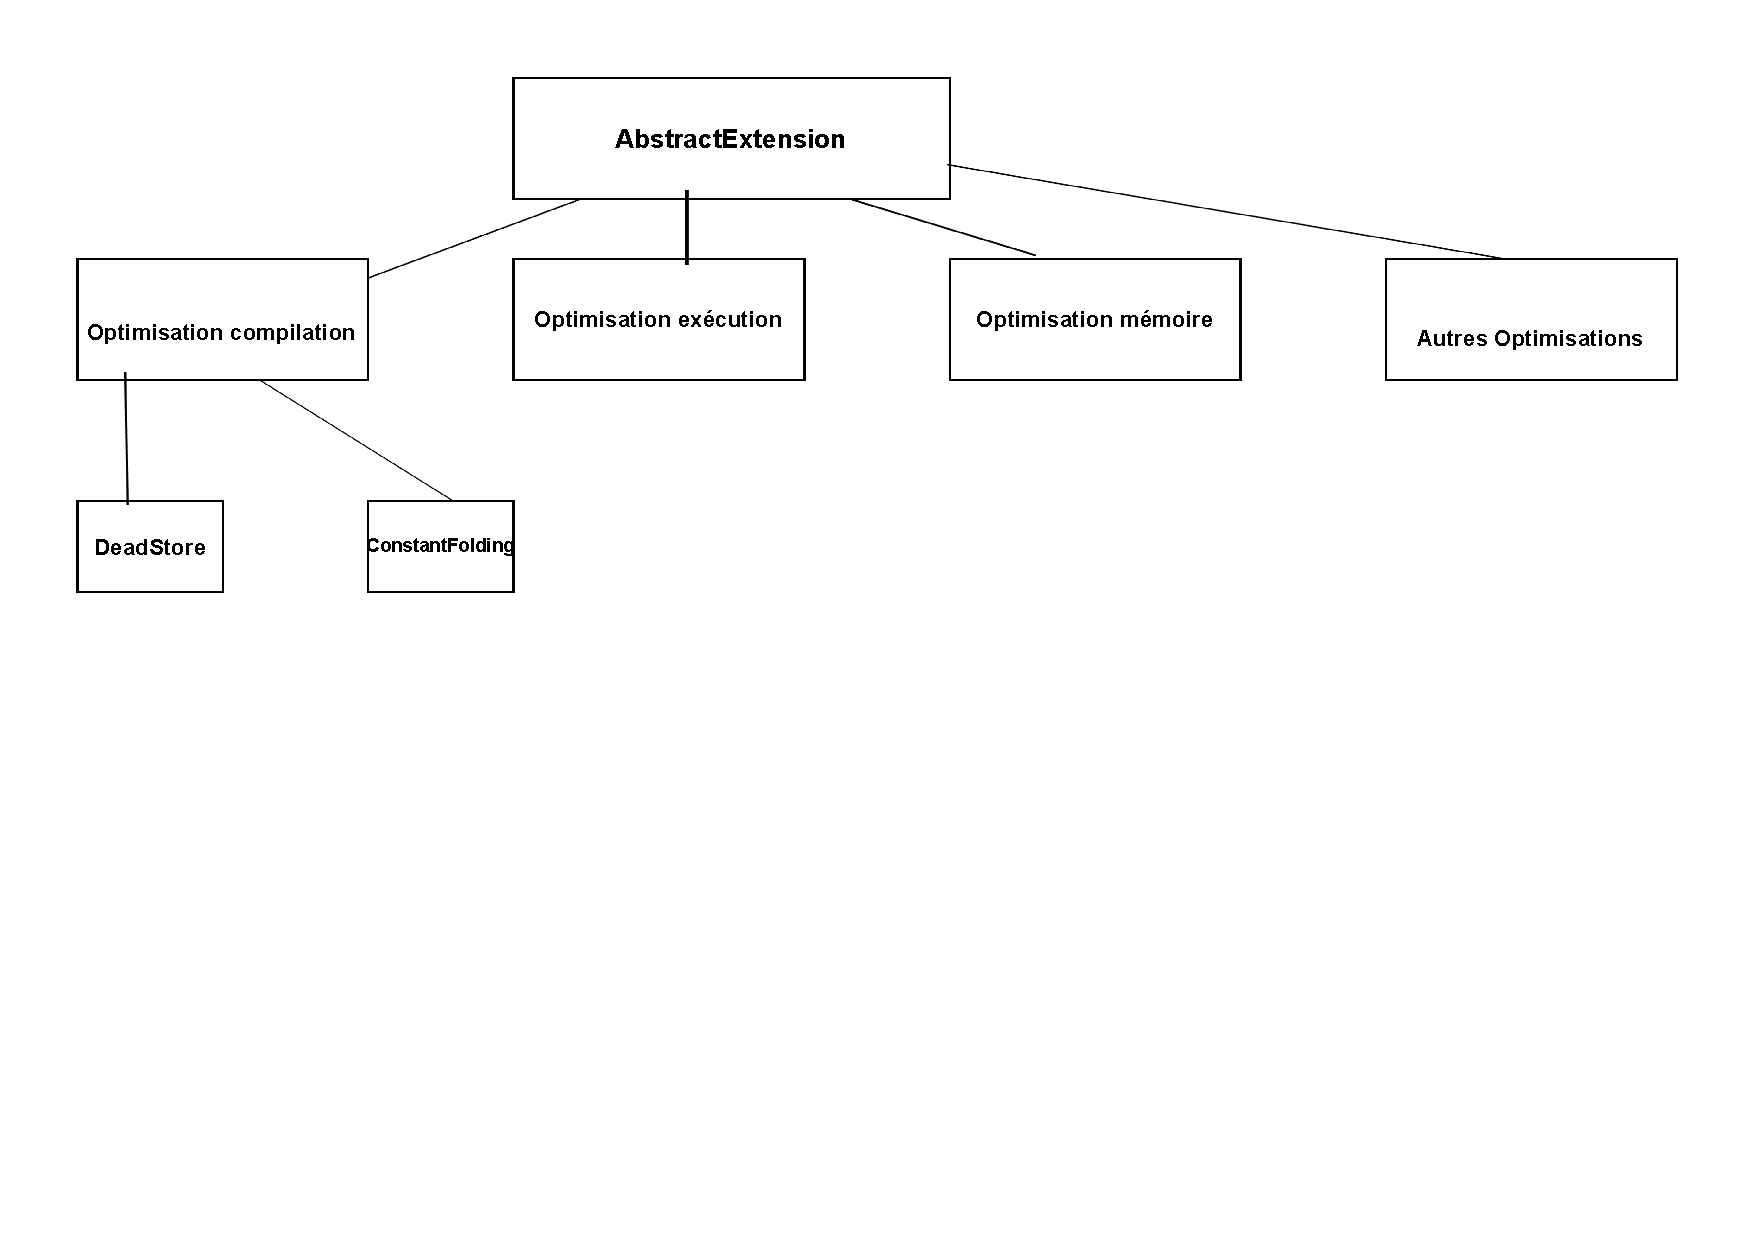
\includegraphics{UML.pdf}\\
Le futur programmeur qui voudra rajouter ses propres optimisations pourra ainsi créer ses propres classes, ses propres dépendances et ajouter les attributs qui lui sembleront nécessaires.

\end{document}
